\documentclass[12pt,a4paper]{article}
\usepackage{mathrsfs}
\usepackage{amsmath}
\usepackage{amsfonts}
\usepackage{amssymb}
%\usepackage{fullpage}
\usepackage{caption}
\usepackage{pdfpages}
\usepackage{subcaption}


\begin{document}

\title{Theoretical study of Axion-Like Particle (ALP) couplings to quarks and gluons, and experimental study of ALP resonances in dijet invariant mass spectrum using Monte Carlo data}
\author{Komal Tauqeer \\ Quaid-i-Azam University, \\Islamabad, Pakistan}
\date{September 20, 2019}

\maketitle

\begin{abstract}

New particles like Axions are very well-motivated in BSM models as gauge-singlets. One can describe their interactions with SM fields by an effective Lagrangain. In this report, we will discuss the study of SM particles specifically quarks and gluons. At the partonic level, the pseudoscalar alp can decay into colored particles. At tree-level the relevant modes are $a \rightarrow g g$ and $a \rightarrow q ̄\bar q$. We will be looking for ALP resonances having mass slightly higher from 1 GeV, specially we will look for 10 GeV, 80 GeV and 350 GeV. We will present the study of ALP decay widths as a function of ALP mass and coupling strength. Also we discuss the expected cross-sections for various processes having combination of ALPs, quarks and gluons as a function of the coupling strengths. Furthermore, we present an experimental study of resonances decaying into two jets using Monte Carlo (MC) data. In this search, we will present the study of parton level, particle level and detector level widths of an ALP having mass 80 GeV and 350 GeV in dijet invariant mass distribution. \\

*References and GitHub repositories will be added in later version. \center{Some parts of this report will be reworded and shortened in the second iteration that will be uploaded to CDS.}

\end{abstract}
\pagebreak

\section{Introduction}
In this report we will present the study of Axion-like particles (ALPs), which are hypothetical elementary particles postulated by the Peccei-Quinn theory in 1977 to resolve the strong CP problem in quantum chromodynamics (QCD). If axions exist and have low mass within a specific range, they are of interest as a possible component of cold dark matter. 
Since axions have a strong theory behind, in order to find their existence we need to understand how they couple to SM particles which includes quarks, gluons, leptons etc. \\
We will study effective lagrangian of such axions having interactions with SM particles and will discuss the decay widths of ALPs into these particles. Furthermore, we will find out the branching ratios of ALPs decaying to quarks and gluons and cross-sections for $ g g \rightarrow a \rightarrow g g $, $g g \rightarrow  a \rightarrow q \bar{q}$, $q \bar{q} \rightarrow  a \rightarrow g g $, $q \bar{q} \rightarrow  a \rightarrow  q \bar{q}$ with ALP as mediator.
When two quarks or gluons collide, it is possible for them to decay into the mediator particle (which is axion for our model). This mediator can decay back into two quarks or gluons, which will be detected as jets in detector. The invariant mass of the two jets will be equal to the mass of the mediator (ALP). Such events, called di-jet, have been examined in this report. The simulated events were generated in MadGraph5. The simulations are divided into different levels. At parton level only the interaction between quarks or gluons is considered. At particle level the creation of jets is simulated and the last level includes how the particles interact with the detector. All Monte Carlo(MC) events generated by MadGraph5 are analysed in MadAnalysis5 and we will summarize the relative widths at each level.


\section{Theoretical Motivation}
New pseudoscalar particles with masses below the electroweak scale appear frequently in well-motivated extensions of the Standard Model (SM). Examples are axions addressing the strong CP problem or pseudoscalar mediators of a new interaction between dark or hidden sectors and the SM. Further, various anomalies can be explained by the presence of new spin-zero states with pseudoscalar couplings. Searches for such resonant enhancements of the dijet invariant mass distribution ($m_{jj}$) are an essential part of the LHC physics programme. New particles like axions with sizeable couplings to quarks and gluons are predicted by many models,including resonances with additional couplings to dark-matter particles.
Searches for dijet resonances with masses of several hundreds of GeV to just above 1 TeV have been carried out at lower-energy colliders and at the LHC, which has also extended search sensitivities into the multi-TeV mass range. In this report, we will specifically study such resonances at three mass points 10 GeV, 80 GeV and 350 GeV with varying coupling to quarks and gluons.


\section{Effective Lagrangian for ALPs}
We assume the existence of a new spin-0 resonance $a$, which is a gauge-singlet under the SM gauge group.  It's mass $m_a$ is assumed to be smaller than the electroweak scale. Then the most  general  effective  Lagrangian  reads 

\begin{equation}
{\mathscr{L}_{eff}}^{D\leq5} = \frac{1}{2} (\partial_\mu a)(\partial^\mu a)- \frac{m^2_{a,0}}{2} a^2 + \frac{\partial ^\mu a}{\Lambda} \sum_F \bar{\psi}_F \textbf{\textit{C}}_F  \gamma_\mu  \psi_F + g^2_s C_{GG} \frac{a}{\Lambda} G_{\mu \nu}^A \tilde{G}^{\mu \nu,A} 
\end{equation}

$$+ g^2 C_{WW} \frac{a}{\Lambda} W_{\mu \nu}^A \tilde{W}^{\mu \nu,A} + {g\prime ^2} C_{BB} \frac{a}{\Lambda}B_{\mu \nu} \tilde{B}^{\mu \nu} 
$$

where $G_{\mu \nu}^A$, $W_{\mu \nu}^A$, $B_{\mu \nu}$ are the field strength tensors of $SU(3)_c$, $SU(2)_L$, $U(1)_Y$ and $g_s$, $g$, $g^{\prime}$ denote the corresponding coupling constant. The dual field strength tensors are defined as $\tilde{B}^{\mu \nu} = \frac{1}{2} \epsilon^{\mu \nu \alpha \beta} B_{\alpha \beta}$

\section{ALP decays to SM particles}
The effective Lagrangian (1) governs the leading interactions (in powers of $(\frac{\upsilon}{\Lambda})$ giving rise to ALP decays into pairs of SM gauge bosons and fermions. We will study tree-level interactions of ALPs with SM particles specifically quarks and gluons.
\subsection{ALP decays to Hadrons}
At the partonic level, the pseudoscalar alp can decay into colored particles. At tree-level the relevant modes are $a \rightarrow g g$ and $a \rightarrow q ̄\bar q$. The decay rate of ALP going to hadrons is given by

\begin{equation}
\Gamma (a \rightarrow hadrons) = \frac{32 \pi \alpha_s^2(m_a) m_a^3}{\Lambda^2}[1 + (\frac{97}{4} - \frac{7n_q}{6}) \frac{\alpha_s(m_a)}{\pi}] \mid C_{GG} + \sum_{q=1}^{n_q} \frac{C_{qq}}{32 \pi^2} \mid ^2
\end{equation}
$$\equiv \frac{32 \pi \alpha_s^2(m_a) m_a^3}{\Lambda^2} [1 + \frac{83}{4} \frac{\alpha_s(m_a)}{\pi}] \mid C_{GG}^{eff} \mid ^2$$

where $n_q = 3$ is the number of light quark flavours and $\alpha_s$ is the coupling strength of strong interaction (QCD) as a function of ALP mass. Its values for different ALP masses is summarized in Table 1. For simplicity we will choose $n_q = 1$ i.e. only "up type" quarks for this study. To good approximation this rate scales with the third power of the ALP mass.  

\section{Theoretical calculation of ALP decay widths}
In this section, we will discuss ALP decay widths into SM quarks and gluons using [2] specifically looking at three different mass points and with varying coupling strengths and try to deduce the dependence of decay rate on coupling strength and mass of an ALP.
\subsection{Decay widths for $a \rightarrow g g, C_G = 1$}
Using equation [2], one can calculate the decay width of ALP into gluons for $C_G = 1$ and $C_{qq} = 0$. See Table 2 below for decay rates for 10 GeV, 80 GeV and 350 GeV mass.\\

\begin{table}
\begin{center}
\label{tab : table1}
\begin{tabular}{l|c|r}
\hline
\textbf{10 GeV} & \textbf{80 GeV} & \textbf{350 GeV} \\
\hline
0.179 &  0.121 &  0.099 \\
\hline
\end{tabular}
\caption{Values of $\alpha_s$ as a function of $m_a$}
\end{center}
\end{table}


\begin{table}[h!]
\begin{center}
\label{tab : table2}
\begin{tabular}{l|c|r}
\hline
\textbf{10 GeV} & \textbf{80 GeV} & \textbf{350 GeV} \\
\hline
0.00744232 GeV & 1.42118 GeV & 72.8637 GeV \\
\hline
\end{tabular}
\caption{ALP decay rates into gluons for $C_G =1$}
\end{center}
\end{table} 


\subsection{Decay widths for $a \rightarrow g g, C_G = \frac{1}{4\pi}$}
Table 3 below shows the  decay rates of ALP into gluons with coupling strength equal to $\frac{1}{4\pi}$, roughly equal to 0.08.

\begin{table}[h!]
\begin{center}
\label{tab : table3}
\begin{tabular}{l|c|r}
\hline
\textbf{10 GeV} & \textbf{80 GeV} & \textbf{350 GeV} \\
\hline
4.76309e-05 GeV & 0.00909555 GeV  & 0.466327 GeV \\
\hline
\end{tabular}
\caption{ALP decay rates into gluons for $C_G =\frac{1}{4\pi}$}
\end{center}
\end{table}

\subsection{Decay widths for $a \rightarrow q \bar{q}, C_{qq} = 1$}
\begin{table}[h!]
\begin{center}
\label{tab : table4}
\begin{tabular}{l|c|r}
\hline
\textbf{10 GeV} & \textbf{80 GeV} & \textbf{350 GeV} \\
\hline
5.77732e-12 GeV & 4.62186e-11 GeV  & 2.02206e-10 GeV \\
\hline
\end{tabular}
\caption{ALP decay rates into quarks for $C_G = 1$}
\end{center}
\end{table}

Table 4 shows the decay width of ALP into quarks with coupling strength equal to 1. For this study we are considering ALP decays to "up type" quarks only.

\section{Calculation of Decay widths of ALP using MadGraph5\_aMC@NLO}
In order to verify theoretically calculated decay rates using [2], we have also calculated decay rates of same processes using MadGraph5. For this purpose we have used a model file which implements effective lagrangain [1]. Summary of decay widths calculated in this manner is shown below.
\subsection{Decay widths for $a \rightarrow g g, C_G = 1$}
Table 5 shows the MadGraph generated decay rates for $a \rightarrow g g, C_G = 1$. \\

\begin{table}[!h]
\begin{center}
\label{tab : table5}
\begin{tabular}{l|c|r}
\hline
\textbf{10 GeV} & \textbf{80 GeV} & \textbf{350 GeV} \\
\hline
0.003214 GeV &  0.751 GeV  & 41.77 GeV  \\
\hline
\end{tabular}
\caption{ALP decay rates into gluons for $C_G =1$ using MadGraph5}
\end{center}
\end{table}

\subsection{Decay widths for $a \rightarrow g g, C_G = \frac{1}{4\pi}$}
Table 6 below shows the MadGraph generated decay rates for $a \rightarrow g g, C_G = \frac{1}{4\pi}$. \\

\begin{table}[!h]
\begin{center}
\label{tab : table6}
\begin{tabular}{l|c|r}
\hline
\textbf{10 GeV} & \textbf{80 GeV} & \textbf{350 GeV} \\
\hline
2.035e-05 GeV & 0.004756 GeV  & 0.2645 GeV  \\
\hline
\end{tabular}
\caption{ALP decay rates into gluons for $C_G =\frac{1}{4\pi}$ using MadGraph5}
\end{center}
\end{table}

\subsection{Decay widths for $a \rightarrow q \bar{q}, C_{qq} = 1$}
\begin{table}[h!]
\begin{center}
\label{tab : table7}
\begin{tabular}{l|c|r}
\hline
\textbf{10 GeV} & \textbf{80 GeV} & \textbf{350 GeV} \\
\hline
7.762e-13 GeV & 7.762e-12 GeV  & 6.209e-11 GeV \\
\hline
\end{tabular}
\caption{ALP decay rates into quarks for $C_G = 1$ using MadGraph5}
\end{center}
\end{table}

Table above shows the MadGraph5 generated decay rates for $a \rightarrow q \bar{q}, C_{qq} = 1$. 

\section{Comparison between theory and MadGraph calculated decay widths}
To make a comparison plot between theoretical and MadGraph5 calculated decay widths we have written a short python code in jupyter. See Appendix A for the complete code. The plot shown below reveals very nice aggreement between theory and Monte Carlo. Also, we can see from the plot that ALP decay width to gluons is much greater than the quarks. This enables us to conclude that majority of the times ALP will decay into gluons rather than quarks. 

\begin{figure}[h!]
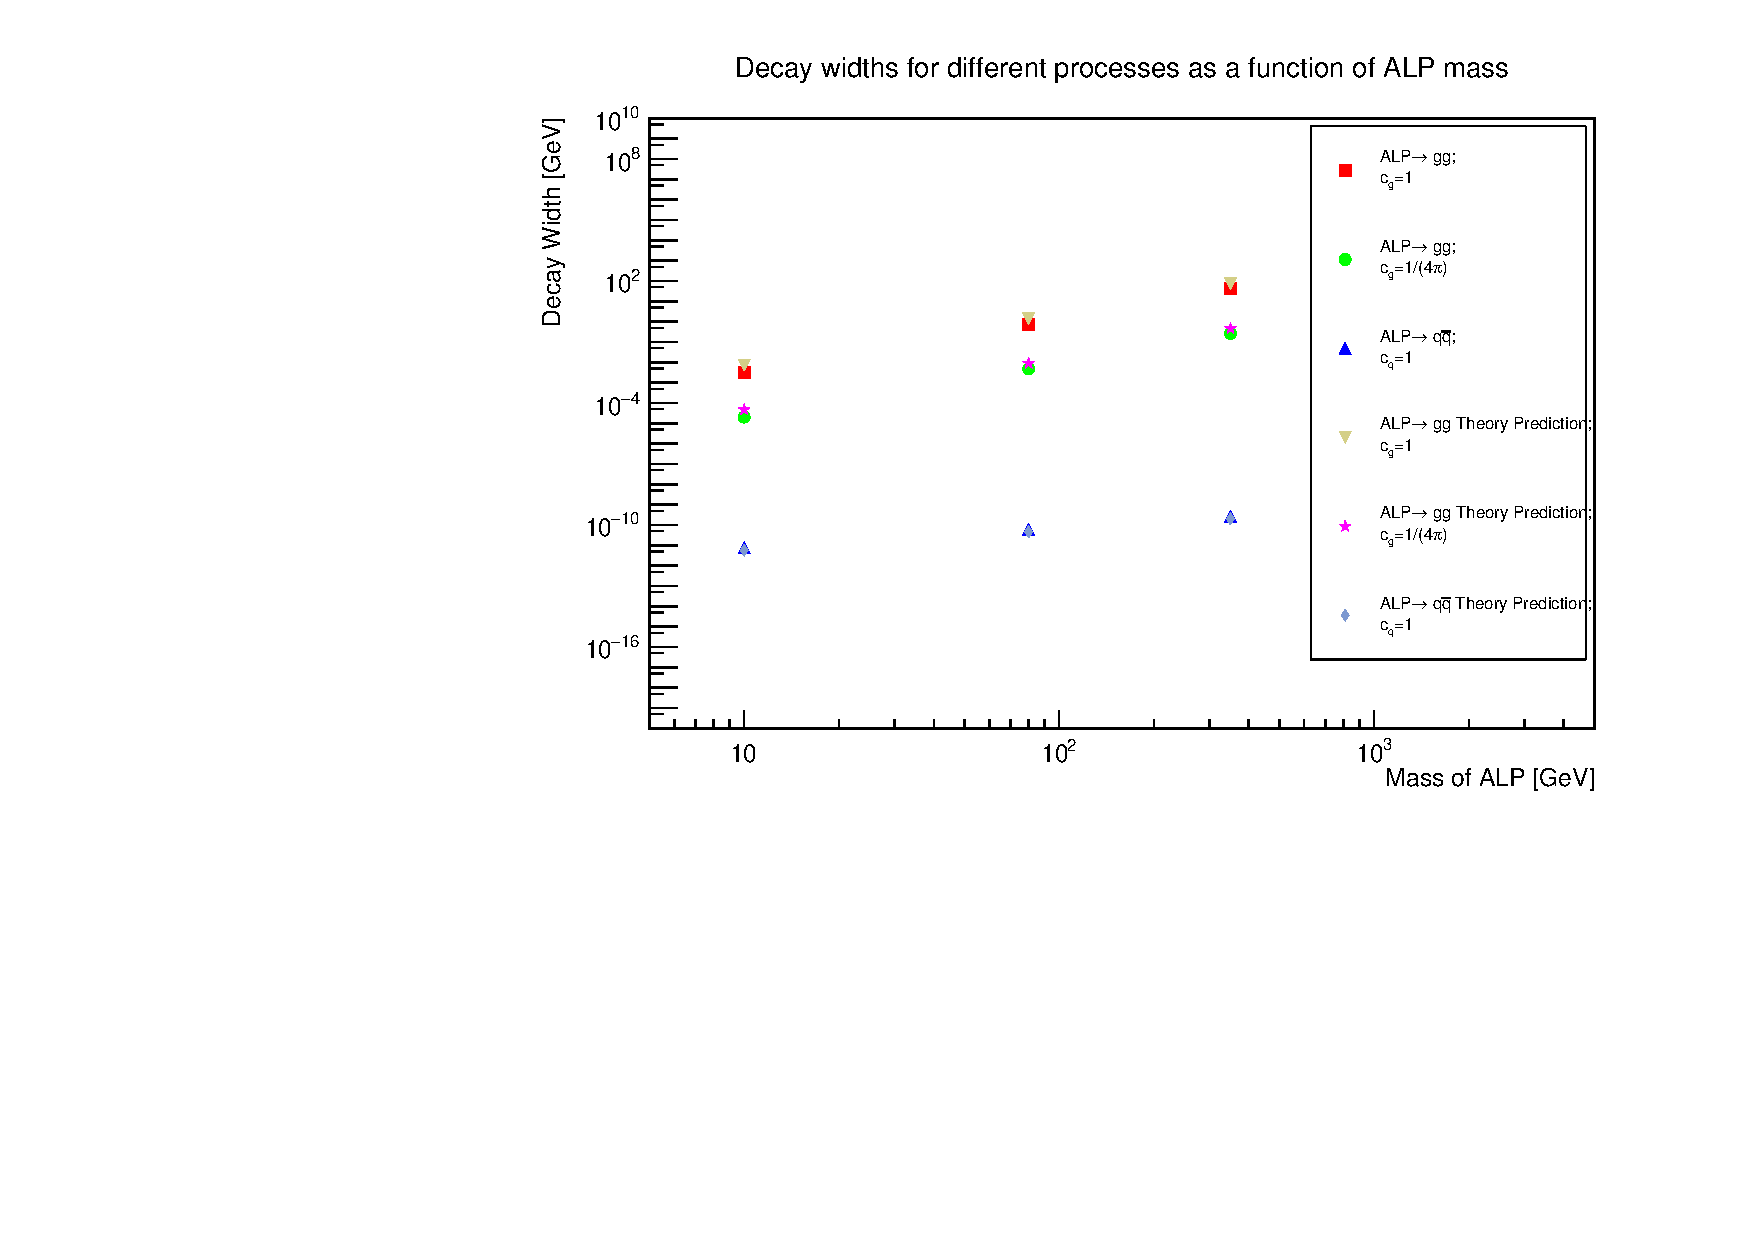
\includegraphics[scale=0.7]{WidthsummaryPlot.pdf}
\caption{ALP decay widths}
\label{fig: figure1}
\end{figure}

\section{Branching Ratios}
Using the calculated decay widths, we have also calculated ALP branching ratios. Summary is given in the tables below.

\begin{table}[h!]
\begin{center}
\label{tab : table8}
\begin{tabular}{l|c|r}
\hline
\textbf{10 GeV} & \textbf{80 GeV} & \textbf{350 GeV}\\
\hline
0.99597 & 0.9990 & 0.94161 \\
\hline
\end{tabular}
\caption{Branching ratios for $a \rightarrow g g, C_G = 1$ }
\end{center}
\end{table}

\begin{table}[h!]
\begin{center}
\label{tab : table9}
\begin{tabular}{l|c|r}
\hline
\textbf{10 GeV} & \textbf{80 GeV} & \textbf{350 GeV}\\
\hline
0.006306 & 0.00632 & 0.005962 \\
\hline
\end{tabular}
\caption{Branching ratios for $a \rightarrow g g, C_G = \frac{1}{4\pi}$ }
\end{center}
\end{table}

\begin{table}[h!]
\begin{center}
\label{tab : table10}
\begin{tabular}{l|c|r}
\hline
\textbf{10 GeV} & \textbf{80 GeV} & \textbf{350 GeV}\\
\hline
2.4053e-09 & 8.2599e-11 & 6.1248e-12 \\
\hline
\end{tabular}
\caption{Branching ratios for $a \rightarrow q \bar{q}, C_{qq} = 1$ }
\end{center}
\end{table}

\section{Expected cross-section for the processes\\ involving ALP, quarks and gluons}

In this section, we will present cross-sections for the possible processes where ALP can couple to gluons and quarks. Feynman diagrams for such processes are shown in figure below.

\begin{figure}[h!]
	\begin{subfigure}{6.5cm}
	\centering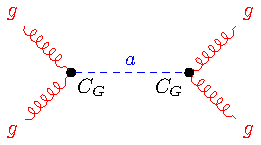
\includegraphics[scale=0.7]{gg_to_gg.pdf}
	\end{subfigure}
	\begin{subfigure}{6.5cm}
	\centering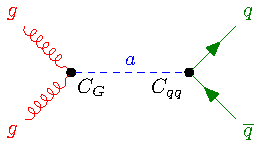
\includegraphics[scale=0.7]{gg_to_qq.pdf}
	\end{subfigure}
	
	\begin{subfigure}{6.5cm}
	\centering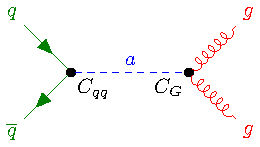
\includegraphics[scale=0.7]{qq_to_gg.pdf}
	\end{subfigure}
	\begin{subfigure}{6.5cm}
	\centering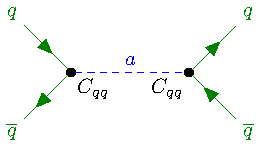
\includegraphics[scale=0.7]{qq_to_qq.pdf}
	\end{subfigure}
\caption{Feynman diagrams}
\label{fig: figure2}
\end{figure}

\subsection{$g g \rightarrow a \rightarrow g g ; C_G = 1$}

\begin{table}[h!]
\begin{center}
\label{tab : table11}
\begin{tabular}{l|c|r}
\hline
\textbf{10 GeV} & \textbf{80 GeV} & \textbf{350 GeV}\\
\hline
1.048e+07 pb & 6.319e+05 pb  & 2.471e+04 pb  \\
\hline
\end{tabular}
\caption{Cross-sections for $g g \rightarrow a \rightarrow g g ; C_G = 1$ }
\end{center}
\end{table}
\pagebreak
\subsection{$g g \rightarrow a \rightarrow g g ; C_G = \frac{1}{4\pi}$}

\begin{table}[h!]
\begin{center}
\label{tab : table12}
\begin{tabular}{l|c|r}
\hline
\textbf{10 GeV} & \textbf{80 GeV} & \textbf{350 GeV}\\
\hline
6.625e+04 pb & 4024 pb  & 161.9 pb  \\
\hline
\end{tabular}
\caption{Cross-sections for $g g \rightarrow a \rightarrow g g ; C_G = \frac{1}{4\pi} $ }
\end{center}
\end{table}

\subsection{$g g \rightarrow a \rightarrow q \bar{q} ; C_G = 1 ; C_{qq} =1 $}

\begin{table}[h!]
\begin{center}
\label{tab : table13}
\begin{tabular}{l|c|r}
\hline
\textbf{10 GeV} & \textbf{80 GeV} & \textbf{350 GeV}\\
\hline
 0.0188 pb & 4.278e-05  pb  & 1.337e-07   pb  \\
\hline
\end{tabular}
\caption{Cross-sections for $g g \rightarrow a \rightarrow q \bar{q} ; C_G = 1 ;C_{qq} =1 $ }
\end{center}
\end{table}



\subsection{$g g \rightarrow a \rightarrow q \bar{q}; C_G = \frac{1}{4\pi}; C_{qq} = 1$}

\begin{table}[h!]
\begin{center}
\label{tab : table14}
\begin{tabular}{l|c|r}
\hline
\textbf{10 GeV} & \textbf{80 GeV} & \textbf{350 GeV}\\
\hline
0.01721 pb & 4.278e-05  pb  & 7.627e-08  pb  \\
\hline
\end{tabular}
\caption{Cross-sections for $g g \rightarrow a \rightarrow q \bar{q} ; C_G = \frac{1}{4\pi} ;C_{qq} =1 $ }
\end{center}
\end{table}


\subsection{$ q \bar{q} \rightarrow a \rightarrow g g ; C_G = 1;C_{qq} =1 $}

\begin{table}[h!]
\begin{center}
\label{tab : table15}
\begin{tabular}{l|c|r}
\hline
\textbf{10 GeV} & \textbf{80 GeV} & \textbf{350 GeV}\\
\hline
0.0001495 pb & 1.233e-06  pb  & 1.333e-08  pb  \\
\hline
\end{tabular}
\caption{Cross-sections for $ q \bar{q} \rightarrow a \rightarrow g g ; C_G = 1;C_{qq} =1 $ }
\end{center}
\end{table}
\pagebreak

\subsection{$ q \bar{q} \rightarrow a \rightarrow g g ; C_G = \frac{1}{4\pi} ;C_{qq} =1 $}

\begin{table}[h!]
\begin{center}
\label{tab : table16}
\begin{tabular}{l|c|r}
\hline
\textbf{10 GeV} & \textbf{80 GeV} & \textbf{350 GeV}\\
\hline
0.0001372 pb & 1.231e-06  pb  & 7.583e-09  pb  \\
\hline
\end{tabular}
\caption{Cross-sections for $ q \bar{q} \rightarrow a \rightarrow g g ; C_G = \frac{1}{4\pi} ;C_{qq} =1 $ }
\end{center}
\end{table}

\subsection{$ q \bar{q} \rightarrow a \rightarrow q \bar{q} ; C_{qq} = 1$}

\begin{table}[h!]
\begin{center}
\label{tab : table17}
\begin{tabular}{l|c|r}
\hline
\textbf{10 GeV} & \textbf{80 GeV} & \textbf{350 GeV}\\
\hline
4.631e-10 pb & 4.121e-12 pb  & 1.44e-17 pb  \\
\hline
\end{tabular}
\caption{Cross-sections for $ q \bar{q} \rightarrow a \rightarrow q \bar{q} ; C_{qq} = 1$ }
\end{center}
\end{table}

\subsection{Summary plot for cross-sections}
To summarize above cross-sections for various processes and varying coupling values we have a summary plot to show, see figure 3. It can be clearly seen that the ALP branching ratios to gluons is much more than the quarks therefore the cross section for $gg \rightarrow a \rightarrow gg$ is much greater than $q\bar{q} \rightarrow a \rightarrow q\bar{q}$.

\begin{figure}[h!]
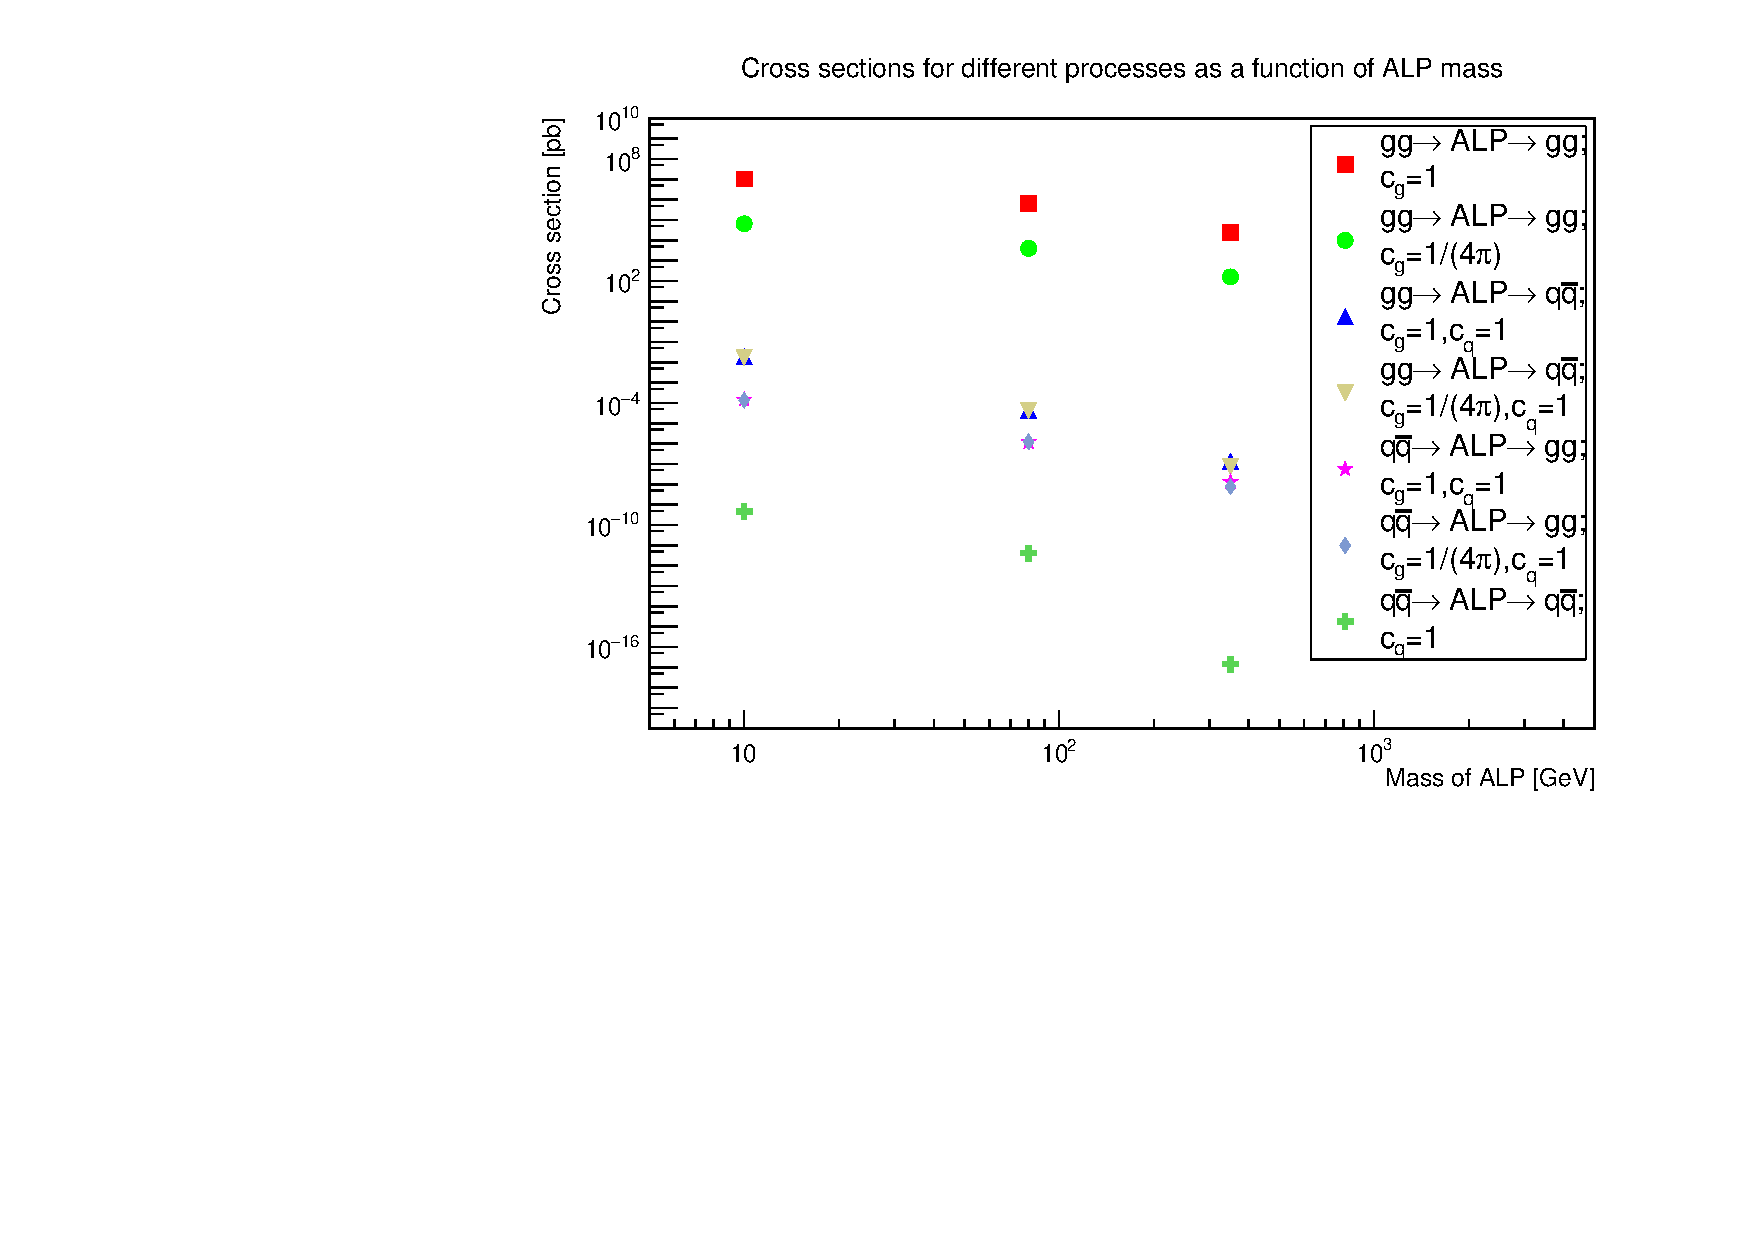
\includegraphics[scale=0.7]{CrossSectionSummaryPlot.pdf}
\caption{Cross-sections of processes including ALP, gluons and quarks}
\label{fig: figure3}
\end{figure}
\pagebreak
\section{Search for ALP resonances in dijet mass distributions}
In this section we will discuss the resonances in invariant mass spectrum at three levels, parton, particle and detector level. We will discuss how such resonances broadens at each level using Monte Carlo data. For this section we will only look for the process $gg \rightarrow a \rightarrow gg ;C_G =1 $ because this process has the highest cross-section amongst the rest discussed in the previous section.


\subsection{Event generation}
The simulated Monte Carlo events are generated using MadGraph5 using model file that implements [1]. 10,000 dijet events were generated for the process $gg \rightarrow a \rightarrow gg; C_G = 1 $ for 80 GeV and 350 GeV ALP at both TRUTH and simulated at the detector level. TRUTH level consists of both the matrix element describing the parton-parton interaction done in MadGraph5 and parton showers (particle level) done in PYTHIA8 as in figure 4. At the detector level, simulation of the interactions of particle with the detector matter is done using Delphes, a software program that simulates particle interactions in matter.

\begin{figure}[h!]
\centering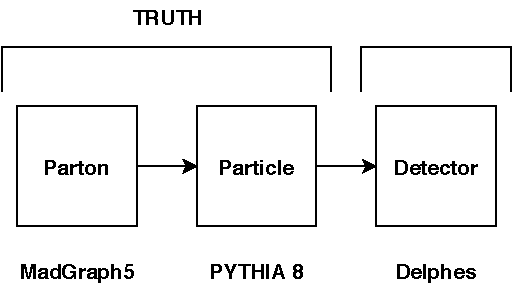
\includegraphics[scale=0.8]{method.pdf}
\caption{The different steps of generating events}
\label{fig: figure4}
\end{figure}


\subsection{Invariant mass distributions}
In order to analyse MC events, MadAnalysis5 was used. We will now present resonances in dijet invariant mass spectrum at each level. Only first two leading partons(for parton level) or jets (for particle and detector level) in $P_T$ are used to calcualte invariant mass using formulla \\ 
$$M^2 = 2P_{{T}_{1}}P_{{T}_{2}}(cosh(\eta_{1} - \eta_{2})-cos(\phi_{1} - \phi_{2})) $$
\subsubsection{Parton-Level distributions}
A resonance at parton level will have a mass given by the energies of the partons. Only the leading two partons in $P_T$ were selected to calculate invariant mass.

\begin{figure}[h!]
	\begin{subfigure}{7.4cm}
	\centering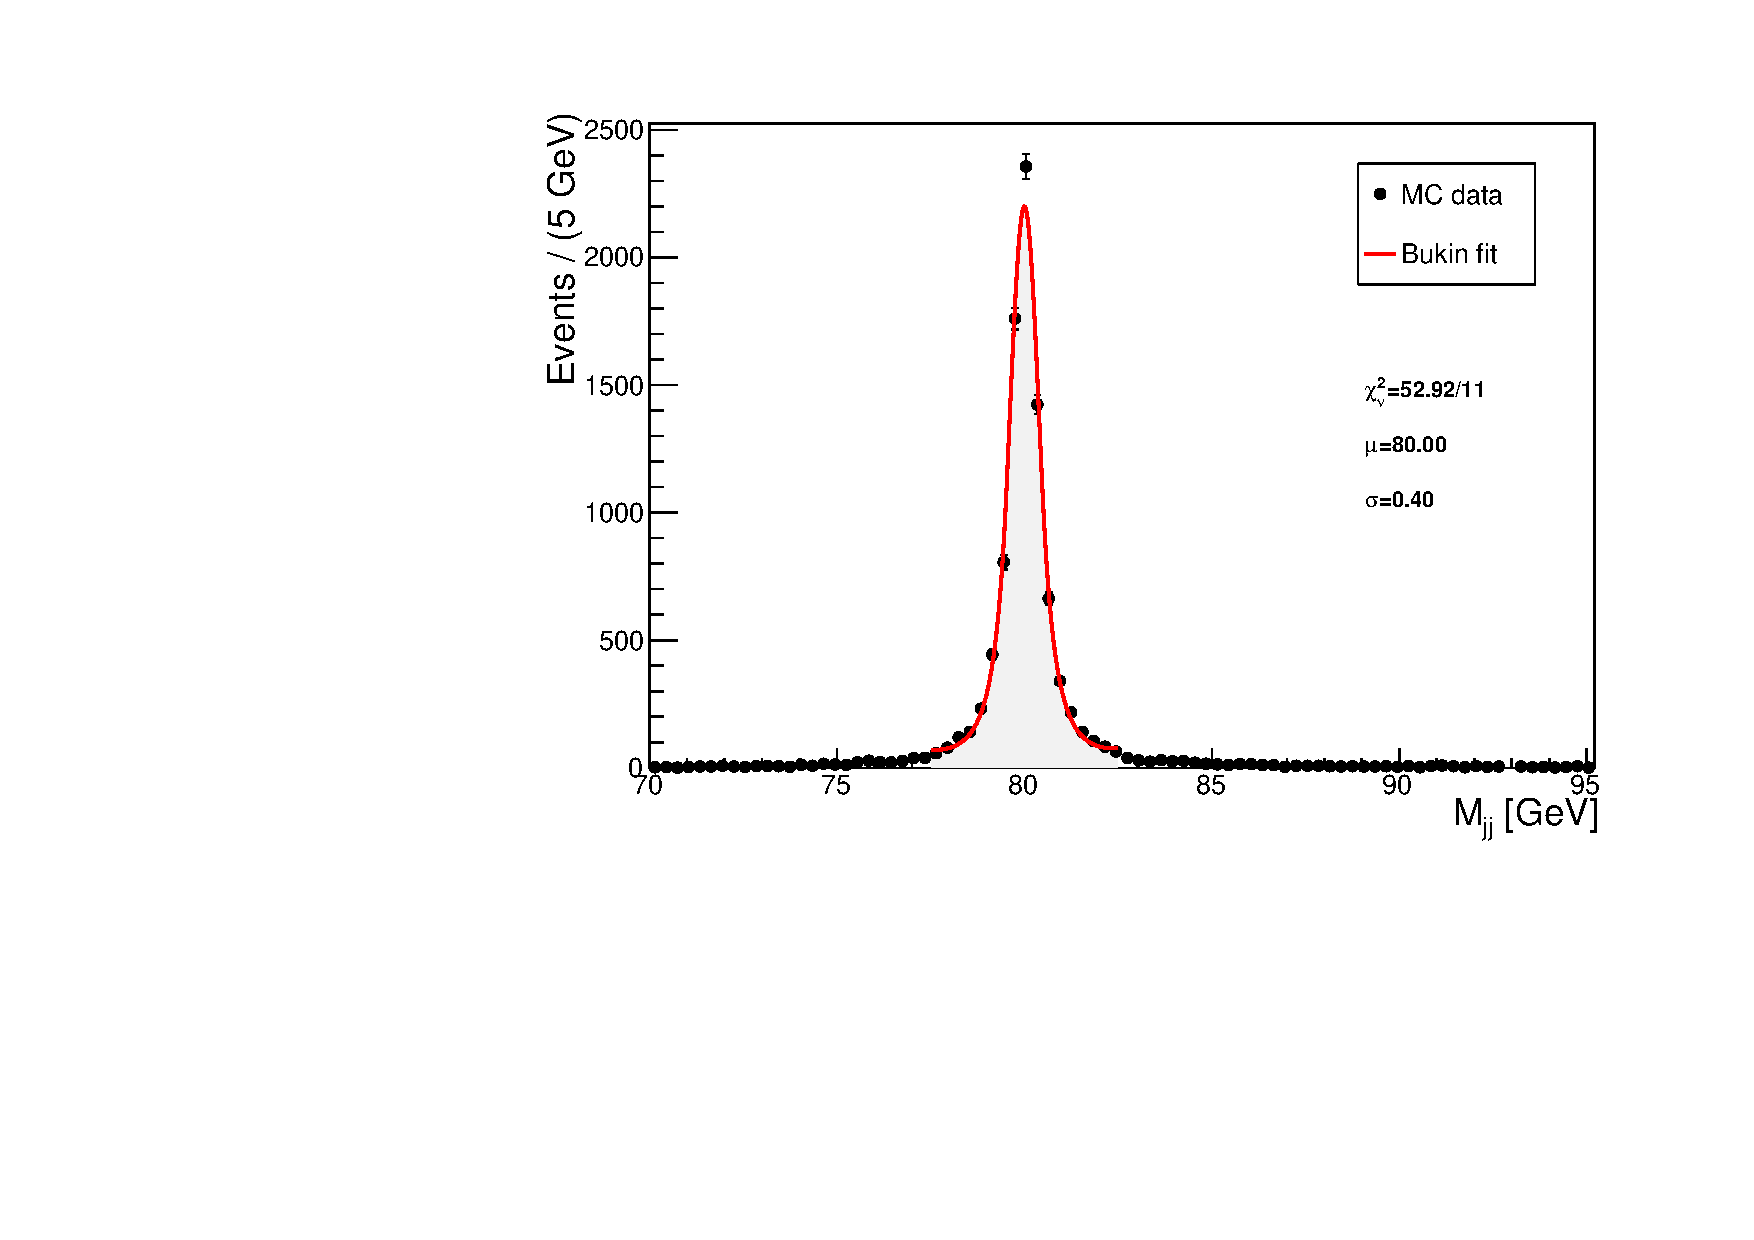
\includegraphics[scale=0.4]{parton_level_80_fit.pdf}
	\end{subfigure}
	\begin{subfigure}{7.4cm}
	\centering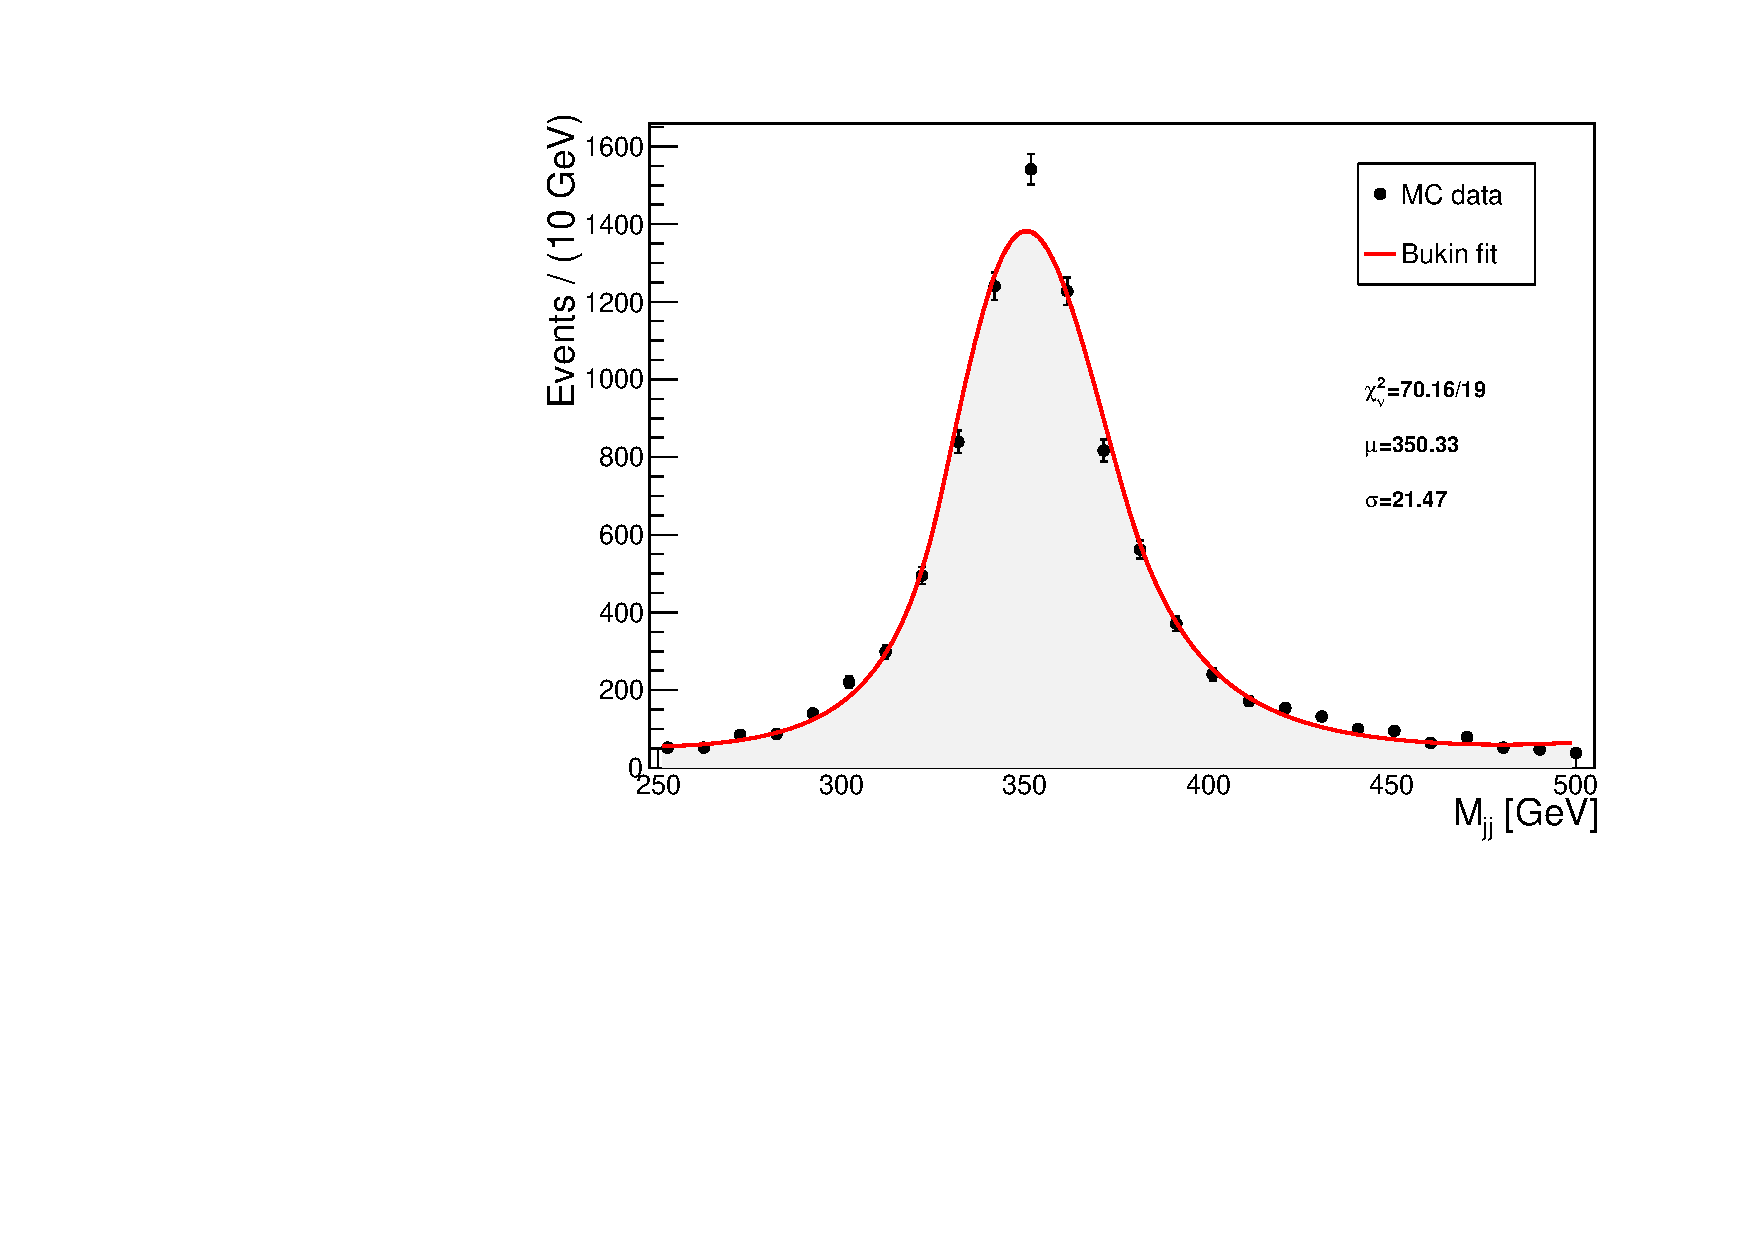
\includegraphics[scale=0.4]{parton_level_350_fit.pdf}
	\end{subfigure}
\caption{Parton level dijet invariant mass distributions for 80 GeV and 350 GeV ALP.}
\label{fig:figure5}	
\end{figure}

\pagebreak


\subsubsection{Particle-Level distributions}
At particle level there will be a smearing to the true particle energy caused by the parton showers. For parton showering we have used PYTHIA8. The resulting event files were reconstructed by anti-$k_t$ algorithm using FastJet simulation requiring $R = 0.4$. Only the leading two reconstructed jets in $P_T$ were selected to calculate invariant mass.

\begin{figure}[h!]
	\begin{subfigure}{7.4cm}
	\centering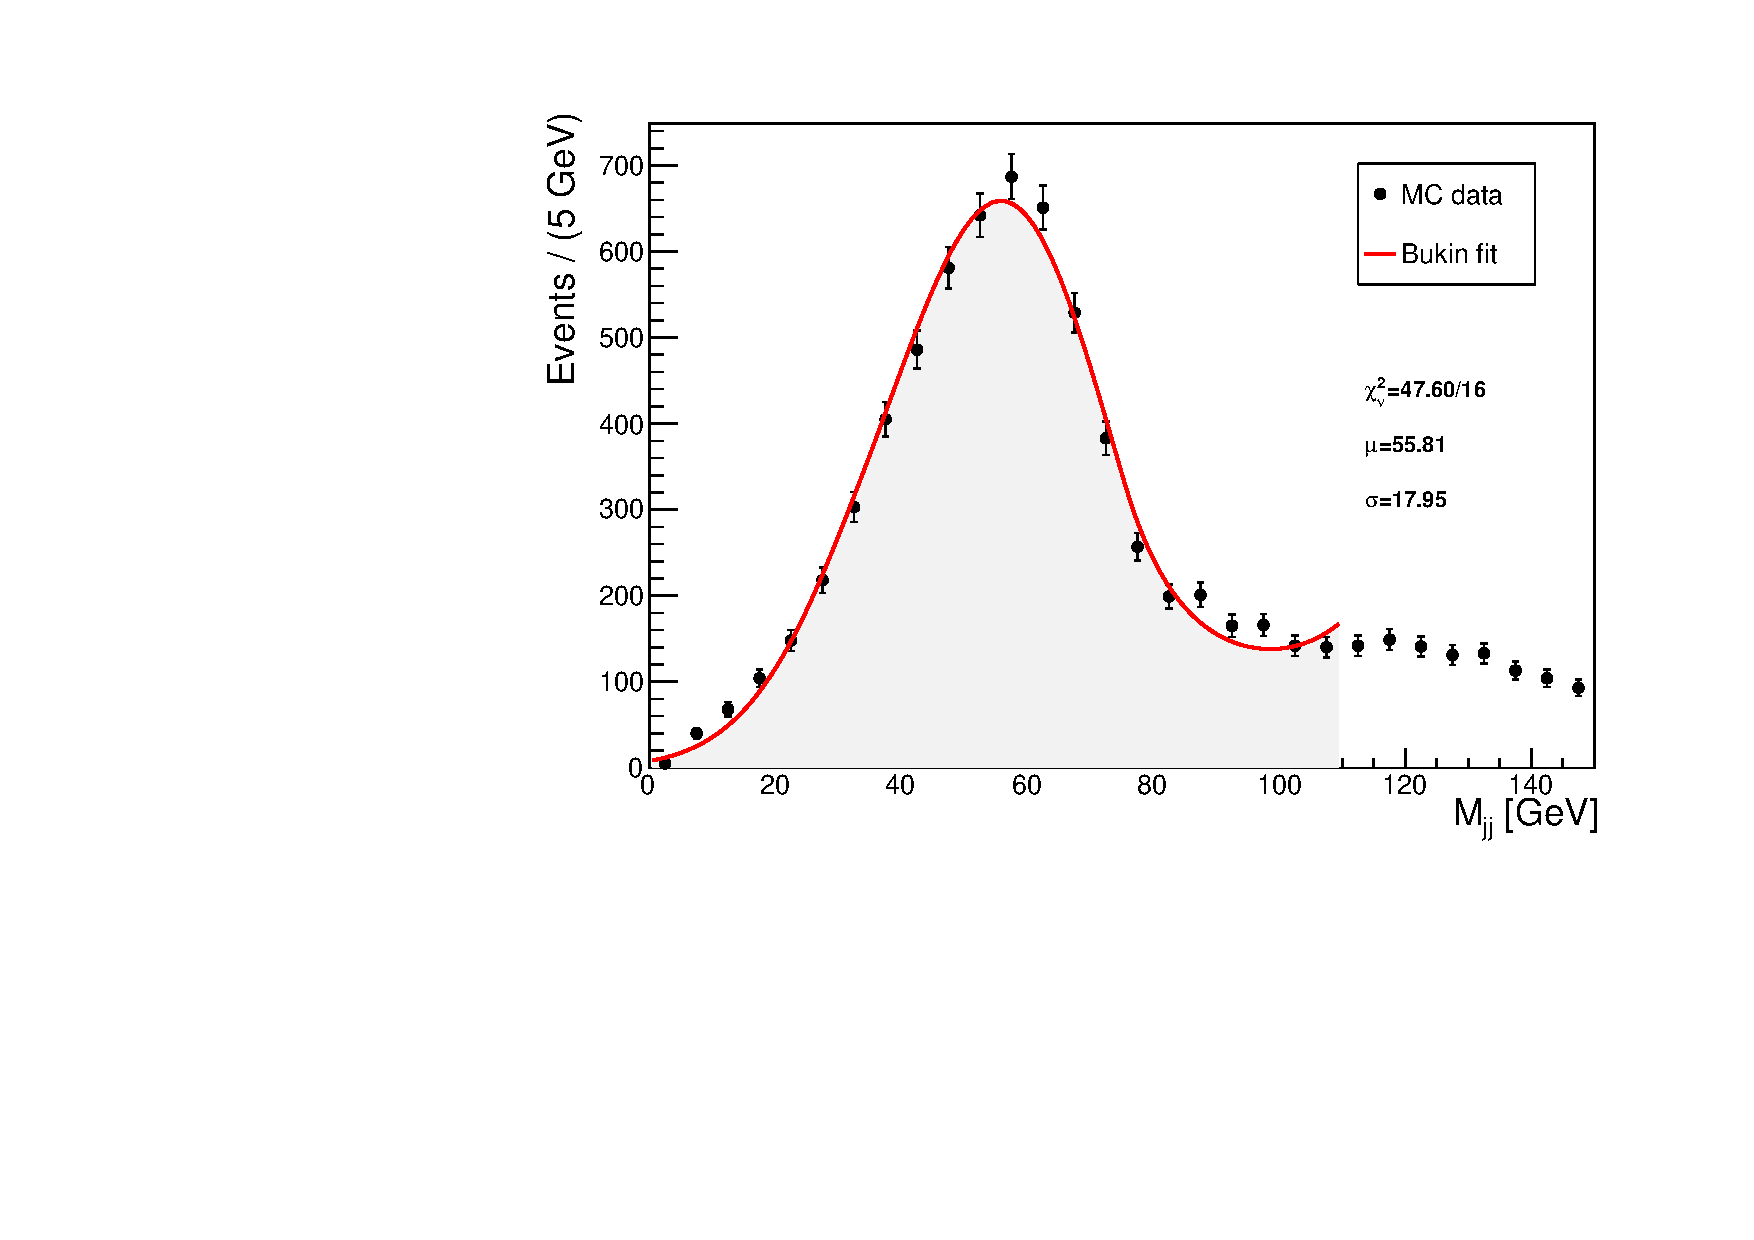
\includegraphics[scale=0.4]{particle_level_80_fit.pdf}
	\end{subfigure}
	\begin{subfigure}{7.4cm}
	\centering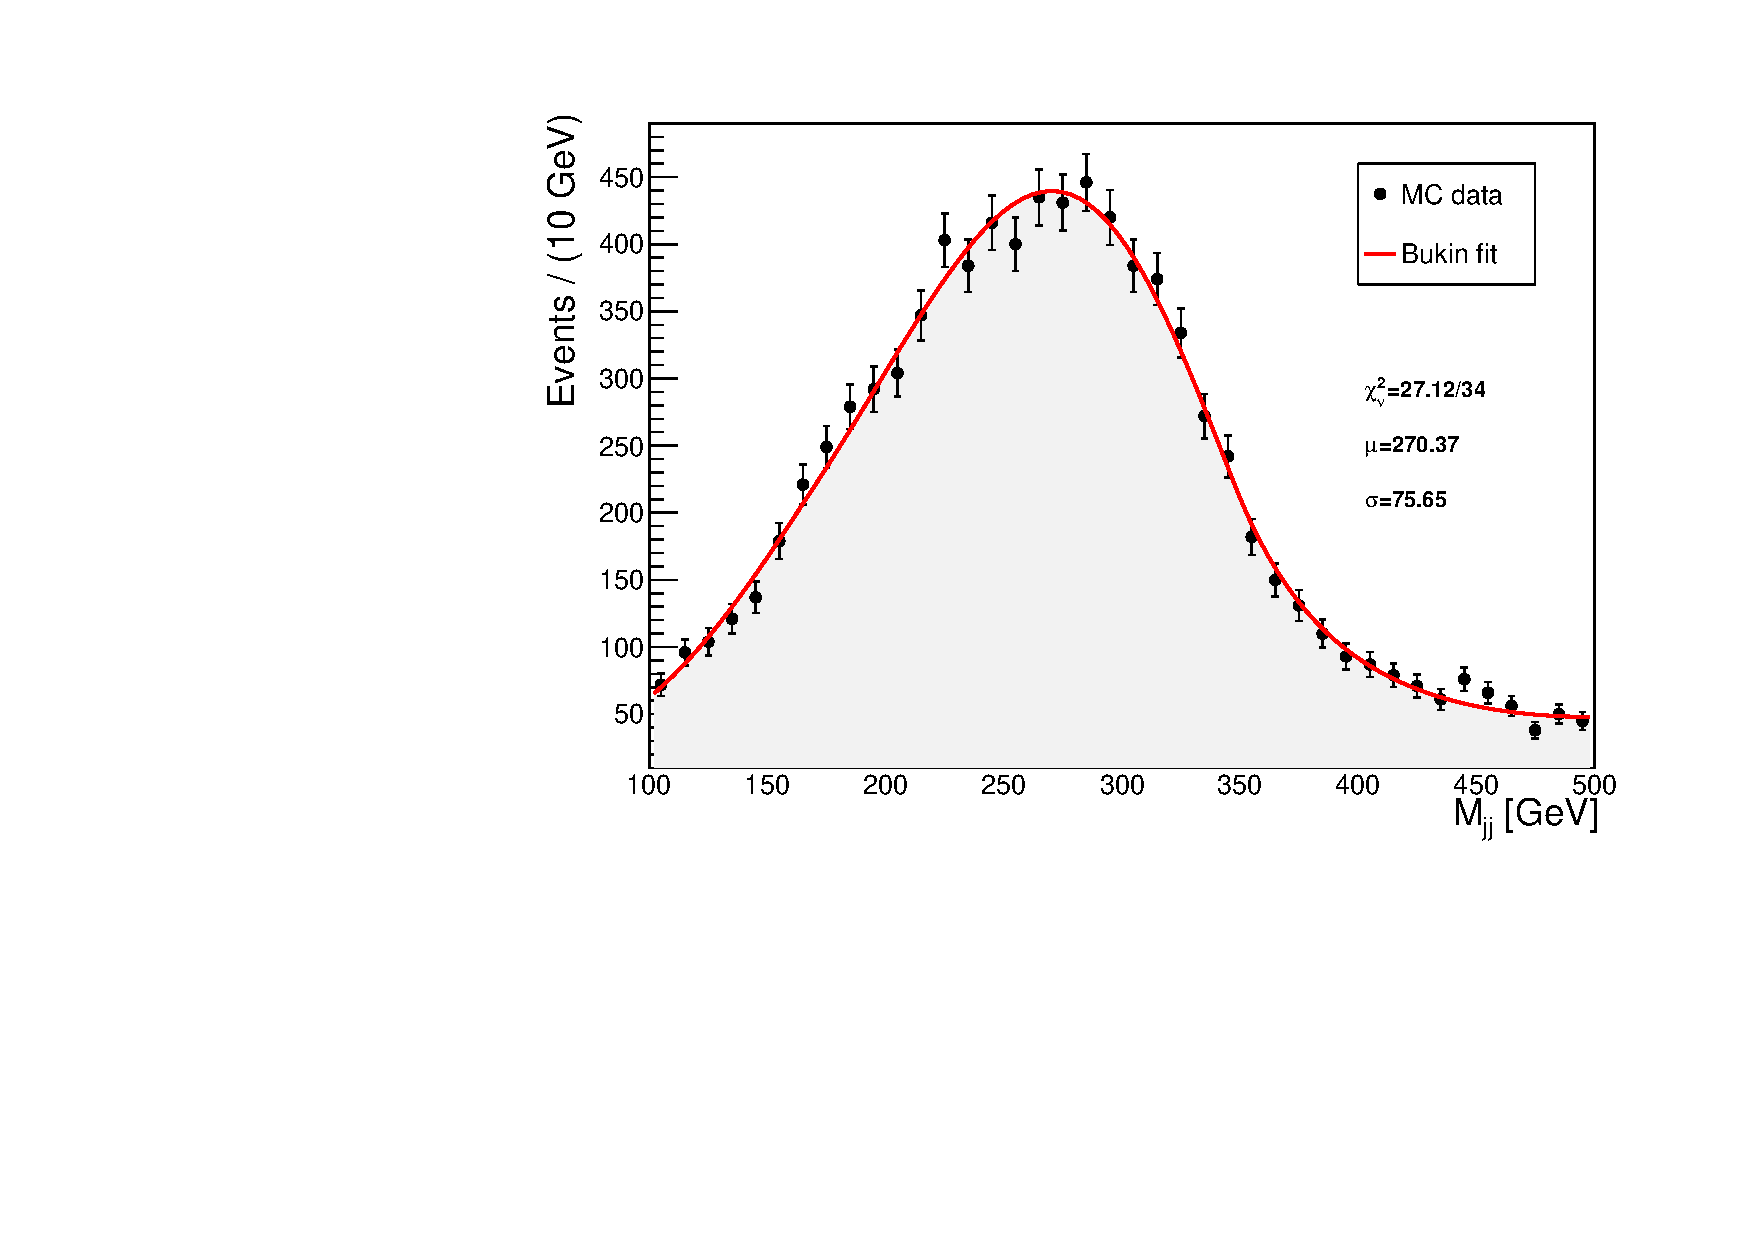
\includegraphics[scale=0.4]{particle_level_350_fit.pdf}
	\end{subfigure}
\caption{Particle level dijet invariant mass distributions for 80 GeV and 350 GeV ALP.}
\label{fig:figure6}	
\end{figure}

\pagebreak

\subsubsection{Detector-Level distributions}
At detector level, measurement of the particles will result in further broadening of the peaks due to the interaction of particles with the matter. For detector simulation and reconstruction we have used Delphes on the MC samples generated by MadGraph5 at parton level and resulting delphes root files were further analysed in expert mode of MadAnalysis5. Only the  leading two reconstructed jets in $P_T$ were selected to calculate invariant mass.

\begin{figure}[h!]
	\begin{subfigure}{7.4cm}
	\centering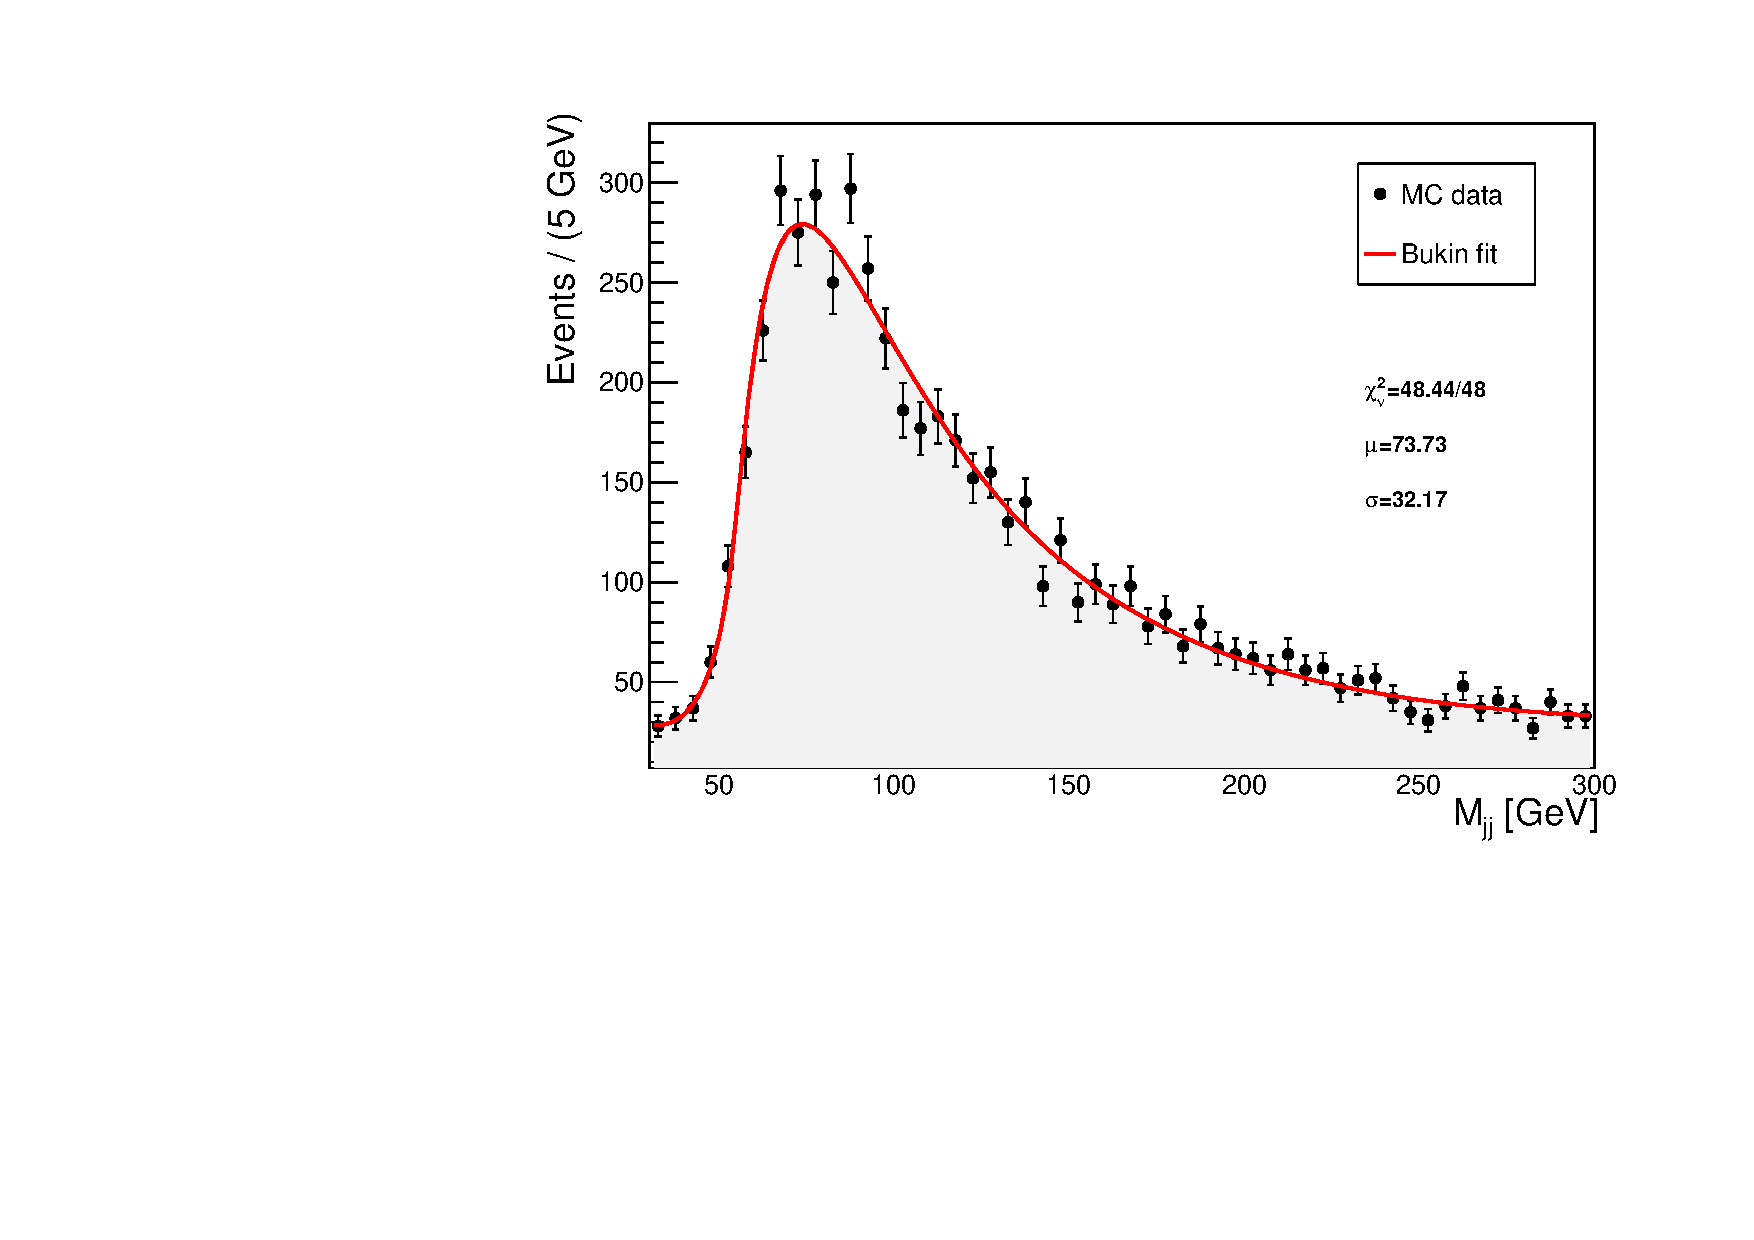
\includegraphics[scale=0.4]{detector_level_80_fit.pdf}
	\end{subfigure}
	\begin{subfigure}{7.4cm}
	\centering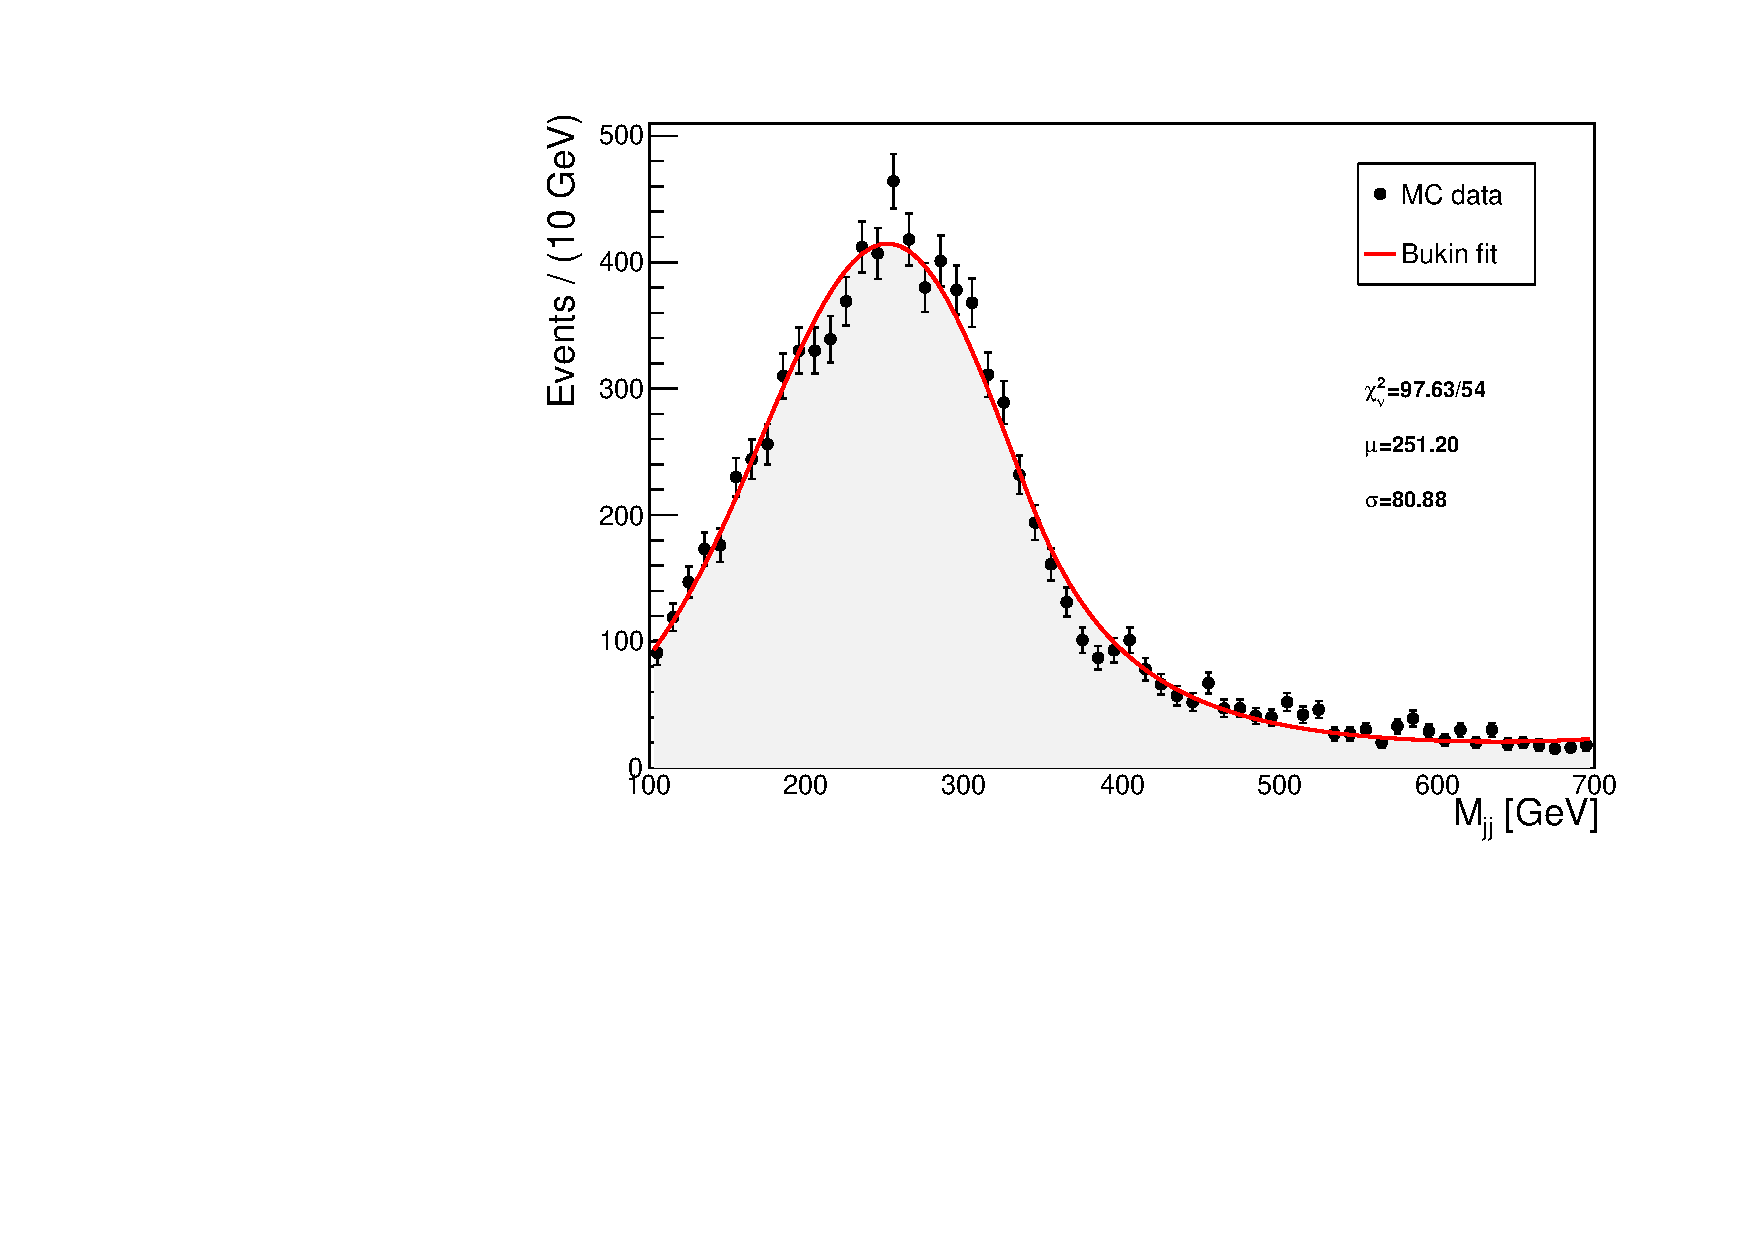
\includegraphics[scale=0.4]{detector_level_350_fit.pdf}
	\end{subfigure}
\caption{Detector level dijet invariant mass distributions for 80 GeV and 350 GeV ALP.}
\label{fig:figure7}	
\end{figure}

\subsection{Relative widths for $g g\rightarrow a \rightarrow g g; C_G = 1$}
Table 18 summarize relative widths of ALP resonance at all three levels and comparison has been made with relative widths calculated from theory.

\begin{table}[h!]
\begin{center}
\label{tab : table18}
\begin{tabular}{l|l|l|l|l}
\hline
\textbf{Mass} & \textbf{Parton Level} & \textbf{Particle level} & \textbf{Detector level} & \textbf{Theory}\\
 & RMS/Mean & RMS/Mean & RMS/Mean & Width/Mass \\
\hline
80 & 0.45/80 = 0.0056 & 16.89/57.7 = 0.29 & 30.8/74.2 = 0.42 & 1.42/80 = 0.018\\
\hline
350 & 84.8/371.5 = 0.23 & 75.6/270.4 = 0.28 & 80/251 = 0.32 & 72.9/350 = 0.21 \\
\hline
\end{tabular}
\caption{Relative widths for $g g\rightarrow a \rightarrow g g; C_G = 1$  }
\end{center}
\end{table}

\pagebreak


\section{Conclusion}
In this report, we have summarized that how the resonance peak broadens from parton level to detector level. This is mainly due to the fact that what we can not measure particles in detector with full accuracy. Also when we take into account hadronization and particle interactions with matter we expect invariant mass peak to be broad. \\
In order to detect new particle like Axions in real data with huge background, it is really important to study well their resonance peaks at MC level and try to find out a way to fnd them in real data by constraining large background.

 

\end{document}